\documentclass{beamer}
\beamertemplatenavigationsymbolsempty
\usecolortheme{beaver}
\setbeamertemplate{footline}[page number]
\setbeamertemplate{itemize item}{\textendash}
\setbeamertemplate{section in toc}[sections numbered]
\usepackage{fontspec}
\setmainfont{cmunrm.otf}[BoldFont=cmunbx.otf,ItalicFont=cmunti.otf,BoldItalicFont=cmunbi.otf]
\setsansfont{cmunss.otf}[BoldFont=cmunsx.otf,ItalicFont=cmunsi.otf,BoldItalicFont=cmunso.otf]
\usepackage[english,russian]{babel}
\usepackage{amsmath,amssymb,booktabs,graphicx,array}
\graphicspath{{figures/}{lab03/figures/}}
\title{The Well: acoustic scattering maze}
\subtitle{Выбор структуры акустического уравнения\\Лабораторная № 3, метод № 4}
\author{}\institute{Foundation models for spatial-time series}\date{14 ноября 2026}
\begin{document}
\begin{frame}\maketitle\end{frame}

\begin{frame}{Две задачи для проверки отбора}\small
Проверяем, как критерий выбирает слагаемые уравнения по наблюдениям давления.
\medskip
\begin{columns}[T]
\begin{column}{.48\textwidth}
\textbf{1. Контрольная задача}\par\medskip
Волна в однородной среде; точное решение известно по формуле.
\begin{itemize}
\item Знаем правильное уравнение.
\item Проверяем лишние ветви.
\item Отдельно добавляем шум.
\end{itemize}
\end{column}
\begin{column}{.48\textwidth}
\textbf{2. The Well: лабиринт}\par\medskip
Опубликованные численные поля в среде со скачками плотности.
\begin{itemize}
\item Сложная геометрия.
\item Производные по кадрам.
\item Перенос на другие траектории.
\end{itemize}
\end{column}
\end{columns}
\medskip
\footnotesize В обеих задачах: одна библиотека из шести слагаемых,
три критерия и семплирование с отклонением.
\end{frame}

\begin{frame}{План презентации}
\tableofcontents[hideallsubsections]
\end{frame}

\section{Пространство моделей и подбор коэффициентов}
\begin{frame}{Из каких слагаемых выбираем модель}\small
\[\boxed{p_{tt}=\sum_{j=1}^{6}s_j\theta_j\phi_j[p;\rho,K]},
\qquad s_j\in\{0,1\}.\]
\footnotesize
\renewcommand{\arraystretch}{1.25}
\begin{tabular}{@{}cl>{\raggedright\arraybackslash}p{4.0cm}@{}}\toprule
$j$ & Возможное слагаемое $\phi_j$ & Смысл\\\midrule
1 & $F_x=K\partial_x(\rho^{-1}p_x)$ & Поток по $x$\\
2 & $F_y=K\partial_y(\rho^{-1}p_y)$ & Поток по $y$\\
3 & $\frac K2[\partial_x(\rho^{-1}p_y)+\partial_y(\rho^{-1}p_x)]$ & Смешанный поток\\
4 & $-p_t/T_0$ & Затухание\\
5 & $-p/T_0^2$ & Линейный возвращающий член\\
6 & $-p^3/(P_0^2T_0^2)$ & Кубическая нелинейность\\\bottomrule
\end{tabular}\par\medskip
$s_j$ выбирает наличие ветви; $\theta_j$ задаёт её коэффициент.
$T_0=1$; $P_0=\max|p_{0,\rm train}|$ одинаков для всех траекторий.
\end{frame}

\begin{frame}{64 структуры и их коэффициенты}\small
\[G=(s_1,\ldots,s_6),\qquad 2^6=64\text{ варианта}.\]
\begin{itemize}
\item Например, $(1,1,0,0,0,0)$ оставляет только $F_x,F_y$;
$(1,1,1,1,1,1)$ включает всю библиотеку.
\item Для каждого $G$ подбираем коэффициенты только по обучению:
\end{itemize}
\[\widehat\theta_G=\arg\min_{\theta_G}\|X_G\theta_G-y\|_2^2.\]
\begin{itemize}
\item Столбцы $X_G$ --- оценки включённых $\phi_j$; $y$ --- оценка $p_{tt}$.
\item Затем решаем PDE из $p_0$ и $p_t(0)=0$ с фиксированной $\widehat\theta_G$.
\item Ищем структуру $G$ и коэффициенты; карты $\rho,K$ известны.
\end{itemize}
\footnotesize Для The Well производные оцениваются по сглаженным данным;
на контрольной задаче они доступны по точной формуле.
\end{frame}

\begin{frame}{Один кандидат: дерево и матрица}
\centering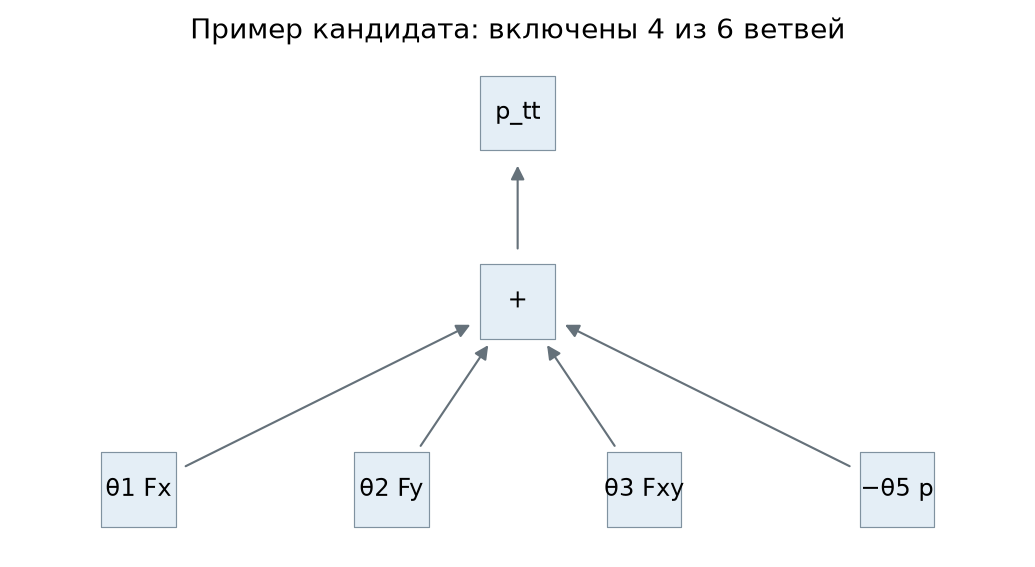
\includegraphics[width=.61\textwidth]{candidate_tree.png}
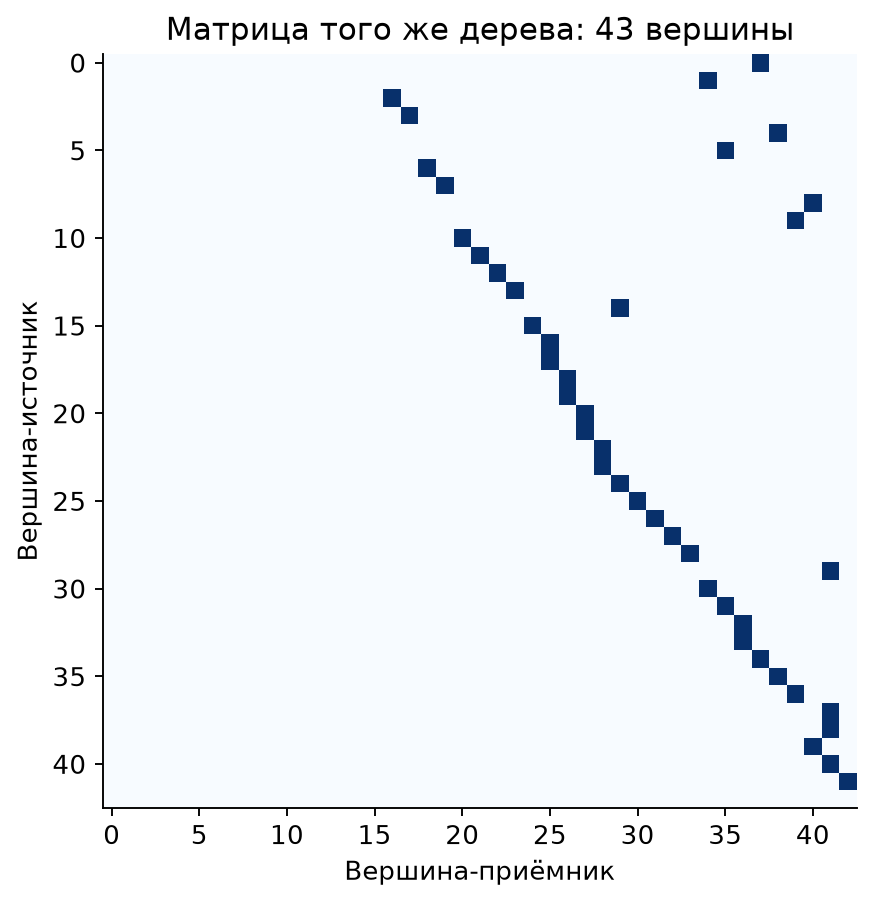
\includegraphics[width=.35\textwidth]{candidate_adjacency.png}\par
\small Пример: $G=(1,1,1,0,1,0)$, четыре включённых слагаемых.\par\medskip
\footnotesize NetworkX хранит дерево выражения и порядок аргументов.
На рисунке ветви сокращены; матрица соответствует полному дереву из 43 вершин.
Это один из кандидатов, а не заранее выбранный ответ.
\end{frame}

\section{Две задачи для проверки отбора}
\begin{frame}{Зачем аналитический бенчмарк}\small
\textbf{Бенчмарк --- контрольная задача с известным ответом.}\par\medskip
Здесь нет лабиринта: однородная среда в квадрате $[0,1]^2$.
\[p_{tt}=c^2(p_{xx}+p_{yy}),\qquad c=0.1.\]
На границе $p=0$; начальная производная $p_t(0)=0$.
\begin{itemize}
\item Знаем нужные члены: $F_x,F_y$ с коэффициентами 1; остальные --- 0.
\item Точное решение даёт давление и производные без разностной оценки.
\item Проверяем поиск сначала без шума, затем с 1\% шума в обучающем $p_{tt}$.
\end{itemize}
\medskip
\footnotesize Одна и та же библиотека кандидатов позволяет проверить критерии
в контролируемых условиях и сопоставить их с опытом на The Well.
\end{frame}

\begin{frame}{Как получаем точный эталон}\small
\[p=\sum_{i,j=1}^{32}A_{ij}\sin(\pi ix)\sin(\pi jy)
\cos\!\left(0.1\pi t\sqrt{i^2+j^2}\right).\]
\begin{itemize}
\item Это сумма колебательных мод; $A_{ij}$ задают начальное поле.
\item Разные $A_{ij}$ дают разные траектории одного уравнения.
\item $A_{ij}$ известны при создании эталона; подбираем другие параметры --- $\theta_j$ модели.
\end{itemize}
\centering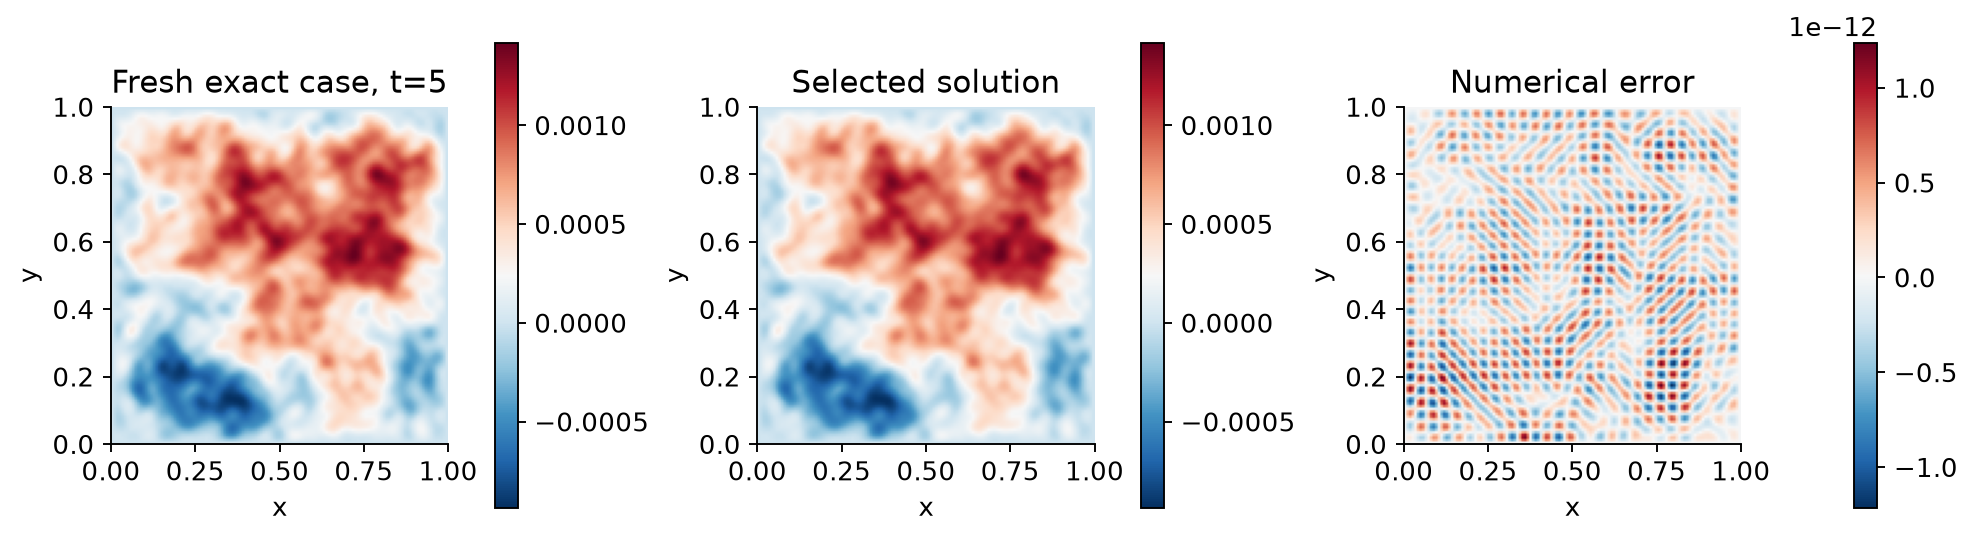
\includegraphics[width=.95\textwidth]{analytic_approximation.png}\par
\scriptsize Точный эталон, численное решение выбранной модели и их разность.
Источник контрольных случаев: \href{https://zenodo.org/records/10406879}{CNO/RPB};
\href{https://arxiv.org/html/2302.01178v2}{Raonić et al., C.3.2}.
\end{frame}

\begin{frame}{The Well: волна в лабиринте}
\centering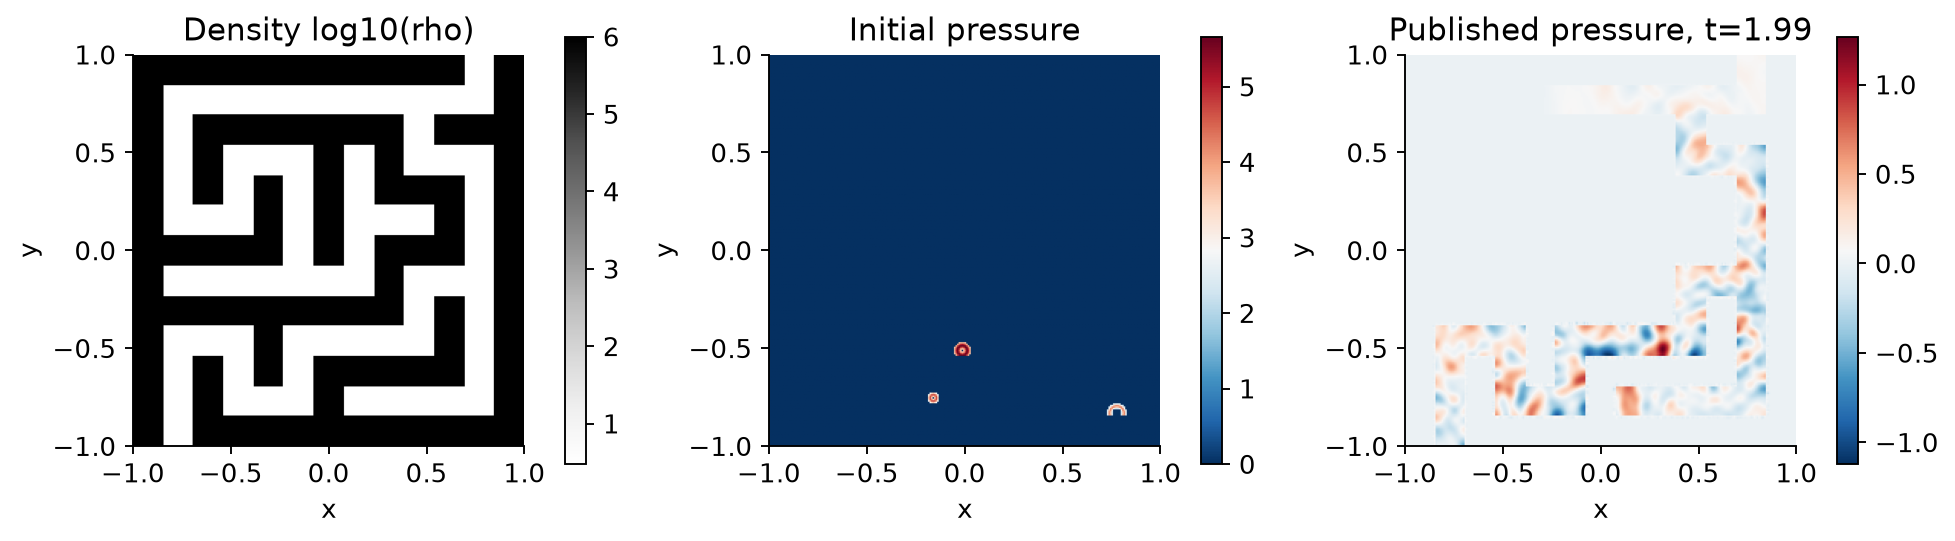
\includegraphics[width=\textwidth]{well_data.png}\par
\small\begin{itemize}
\item Наблюдаем $p(x,y,t)$; известны карты $\rho,c$ и $K=\rho c^2\approx4$.
\item Данные: по 101 кадру на сетке $256\times256$, две координаты и время.
\item Одна траектория для обучения, одна для валидации, две для переноса;
отдельная общая тестовая траектория.
\end{itemize}
\scriptsize\href{https://huggingface.co/datasets/polymathic-ai/acoustic_scattering_maze}{The Well: опубликованные симуляции Clawpack}, не физические измерения.
\end{frame}

\section{Составляющие оценки и три критерия}
\begin{frame}{Составляющие оценки: точность}\small
\textbf{Ошибка давления на основной валидации}
\[E_p(G)=\frac{\|p_G-p_{\rm val}\|_2}{\|p_{\rm val}\|_2}.\]
Сравниваем прямое численное решение с полями в пространстве и времени.\par\medskip
\textbf{Ошибка дифференциальных моментов}
\[E_m(G)=\frac{\|X_{\rm val}\widehat\theta_G-y_{\rm val}\|_2}{\|y_{\rm val}\|_2}.\]
Проверяем выполнение уравнения на оценках производных. Это другая ошибка.\par\medskip
\textbf{Ошибка переноса на две другие траектории}
\[E_{\rm int}(G)=\frac12\sum_{k=1}^{2}
\frac{\|p_G^{(k)}-p_{\rm ref}^{(k)}\|_2}{\|p_{\rm ref}^{(k)}\|_2}.\]
\footnotesize Коэффициенты не переподбираются. Эталоны --- собственные поля новых
траекторий. Тест в эти оценки не входит; ошибки в J используются в долях.
\end{frame}

\begin{frame}{Сложность и оценка присутствия ветвей}\small
\textbf{Число включённых слагаемых}
\[N(G)=\sum_{j=1}^6s_j.\]
Штраф за N выражает предпочтение простоты; правильное число ветвей не задаётся.\par\medskip
\textbf{Статистическая диагностика из лабораторной № 2}
\begin{itemize}
\item 1000 bootstrap-реплик, блоки 4/8/12 кадров, 95\%-е интервалы коэффициентов.
\item Повторно подбираем коэффициенты без ветви; проверяем рост ошибки и устойчивость к шуму.
\end{itemize}
Пусть $b_j=1$, если диагностика советует сохранить ветвь.
\[B(G)=\frac16\sum_{j=1}^6(1-s_j)b_j.\]
\footnotesize B --- мягкий штраф за удаление таких ветвей. Метка диагностики
может отражать численную систематику и не доказывает физическое присутствие.
\end{frame}

\begin{frame}{Общий и статистический фильтры}\small
\begin{columns}[T]
\begin{column}{.48\textwidth}
\textbf{Общий $I_{\rm num}$}\par\medskip
Одинаков во всех трёх вариантах.
\begin{itemize}
\item Пространственный оператор допустим:
\end{itemize}
\[\theta_1,\theta_2\ge0,\quad \theta_3^2\le4\theta_1\theta_2.\]
\begin{itemize}
\item Устойчивый прямой расчёт.
\item Основная ошибка $E_p\le50\%$.
\end{itemize}
\end{column}
\begin{column}{.48\textwidth}
\textbf{Дополнительный $I_{\rm stat}$}\par\medskip
Возвращаем только в варианте 3.
\[I_{\rm stat}(G)=\prod_{j:\,b_j=1}s_j.\]
\begin{itemize}
\item Все ветви с $b_j=1$ обязательны.
\item Их удаление запрещено независимо от ошибки давления.
\item У допущенных графов $B=0$.
\end{itemize}
\end{column}
\end{columns}
\medskip
\footnotesize Варианты 1/2 используют диагностику мягко через B;
вариант 3 превращает ту же оценку присутствия в жёсткое вето.
\end{frame}

\begin{frame}{Три комбинации одного набора оценок}\small
\[Q(G)=E_p(G)+0.1E_m(G)+0.5E_{\rm int}(G).\]
\renewcommand{\arraystretch}{1.7}
\begin{tabular}{@{}lll@{}}\toprule
Вариант & Целевая функция & Допуск\\\midrule
1. Со сложностью & $J_1=Q+0.02N+0.01B$ & $I_{\rm num}$\\
2. Без сложности & $J_2=Q+0.01B$ & $I_{\rm num}$\\
3. Без N + фильтр & $J_3=Q+0.01B$ & $I_{\rm num}I_{\rm stat}$\\\bottomrule
\end{tabular}\par\medskip
\begin{itemize}
\item В варианте 3 у допущенных графов $B=0$.
\item Отличаются только штраф за N и статистическое вето.
\item Данные, обученные коэффициенты, солвер и остальные веса одинаковы.
\end{itemize}
\footnotesize Веса фиксированы для этого сравнения. Малый J означает предпочтительный
граф внутри конкретного варианта; значения разных J напрямую не сопоставляем.
\end{frame}

\section{Сэмплирование с отклонением}
\begin{frame}{Как сэмплируем структуры}\small
Для каждого варианта используем его J и фильтр I.
\begin{enumerate}
\item Независимо предложить $G\sim\mathrm{Uniform}\{0,\ldots,63\}$.
\item Проверить $I(G)=1$; взять заранее рассчитанную оценку J.
\item Сгенерировать независимое $U\sim\mathcal U(0,1)$.
\item Принять граф при $U\le e^{-J(G)/T}$; иначе отклонить.
\end{enumerate}
\[P(G\mid\text{принят})=
\frac{q(G)I(G)e^{-J(G)/T}}{\sum_Hq(H)I(H)e^{-J(H)/T}}.\]
\footnotesize $J\ge0$, поэтому вероятность принятия не выше 1.
3 раунда по 5000 предложений; маски, U и температуры совпадают между вариантами.
Внутри раунда T фиксирована. Коэффициенты задаёт МНК, не сэмплер.
\end{frame}

\begin{frame}{Пример выборки для критерия 1}
\centering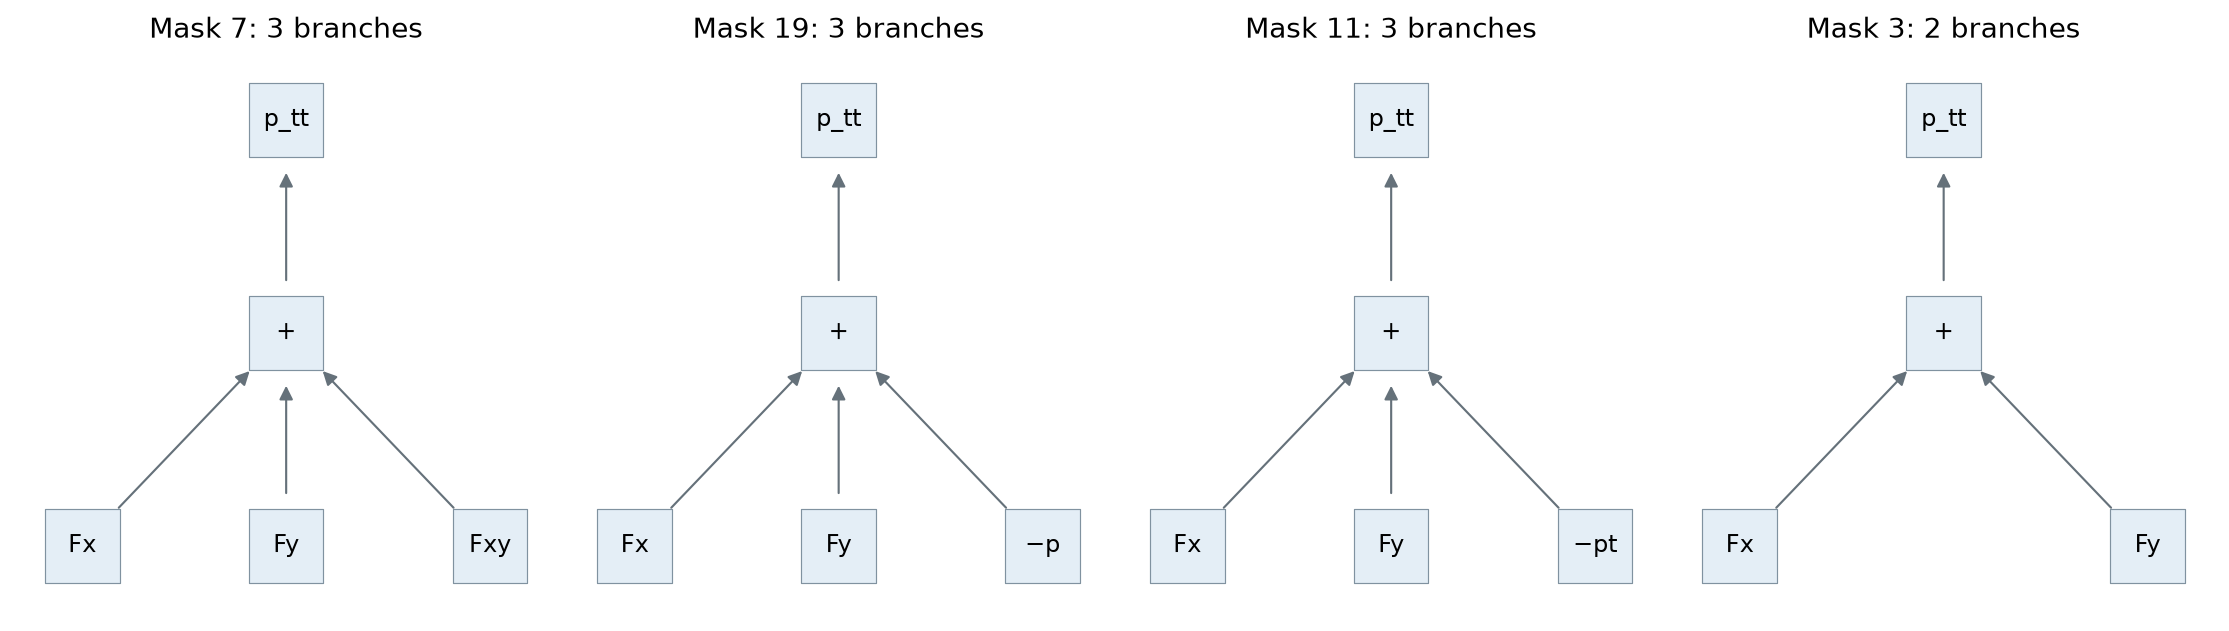
\includegraphics[width=\textwidth]{well_sequence.png}\par
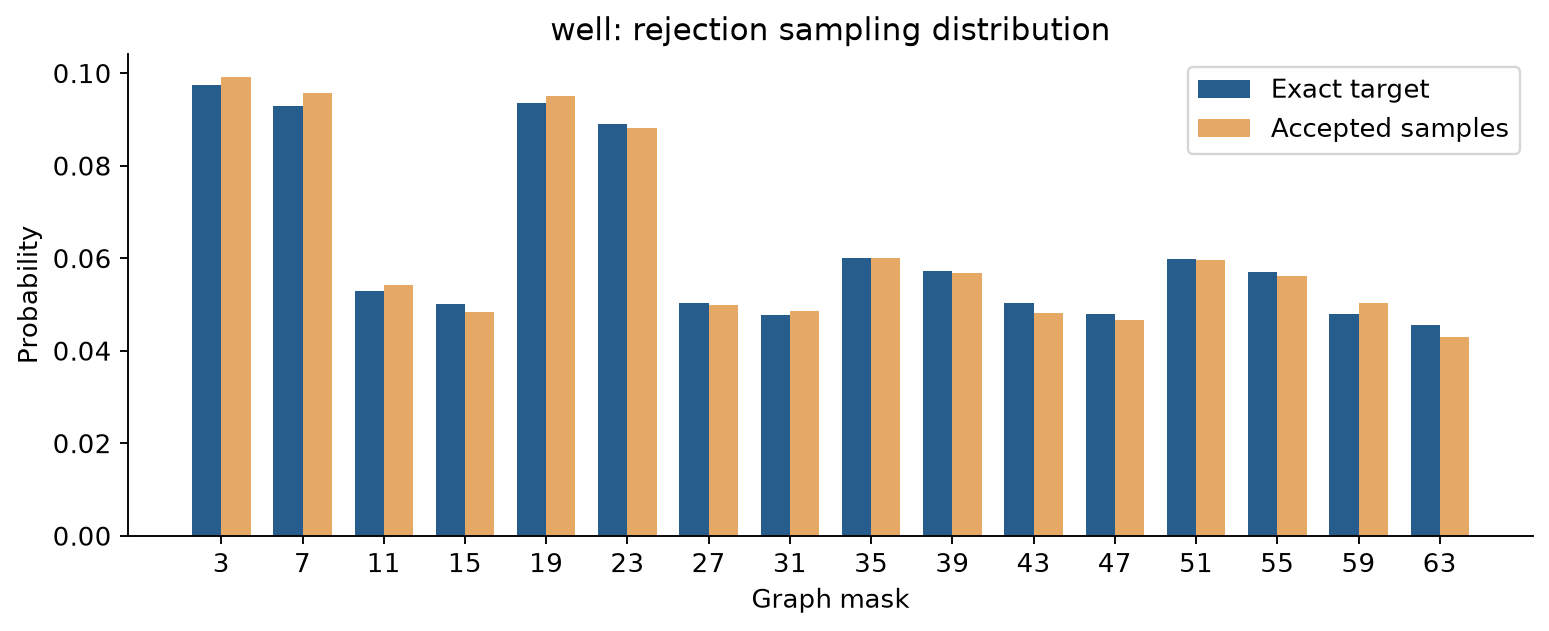
\includegraphics[width=.72\textwidth]{well_distribution.png}\par
\footnotesize Первые три различных принятых графа; справа --- выбранный.
Это независимые предложения, а не последовательное удаление ветвей.
Сохраняем предложения и отказы; минимум каждого критерия проверяем перебором.
\end{frame}

\section{Результаты и сравнение критериев}
\begin{frame}{The Well: результаты трёх критериев}\small
\centering
\renewcommand{\arraystretch}{1.5}
\begin{tabular}{@{}lrrrr@{}}\toprule
Вариант & Ветвей & Валидация & Перенос & Общий тест\\\midrule
1. Со сложностью & 2 & 8.37\% & 7.78\% & 8.21\%\\
2. Без сложности & 4 & 8.00\% & 7.64\% & 8.23\%\\
3. Без N + фильтр & 5 & 22.84\% & 22.87\% & 23.22\%\\\bottomrule
\end{tabular}\par\medskip
\begin{itemize}
\item Штраф выбирает простоту при немного большей валидационной ошибке.
\item Первые два варианта почти одинаковы на общем тесте.
\item Исходный фильтр заметно ухудшает воспроизведение давления в этом опыте.
\end{itemize}
\footnotesize Общая тестовая траектория уже просматривалась: сравнение постфактум.
По одному тесту разницу 8.21\% и 8.23\% нельзя объявлять значимой.
\end{frame}

\begin{frame}{Какие слагаемые выбрали критерии}
\centering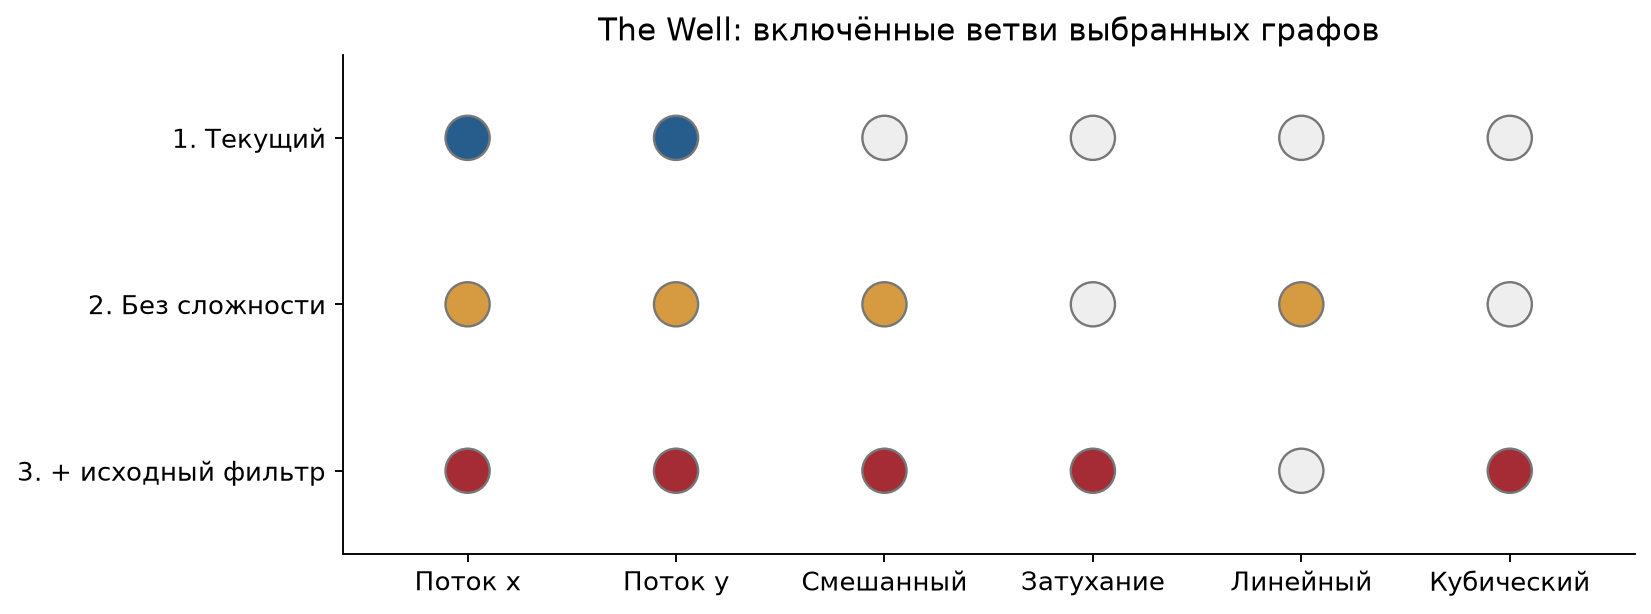
\includegraphics[width=\textwidth]{criterion_variants_branches.png}\par
\small Вариант 1: два потока. Вариант 2: добавлены смешанный и линейный члены.\par\medskip
\footnotesize В варианте 3 диагностика требует затухание: графы без него
запрещены даже при меньшей ошибке. Без штрафа за N сохраняются ещё
смешанный и кубический члены; всего пять ветвей.
\end{frame}

\begin{frame}{Результаты на контрольной задаче}\small
\centering
\renewcommand{\arraystretch}{1.5}
\begin{tabular}{@{}lrrrr@{}}\toprule
 & \multicolumn{2}{c}{Точные данные} & \multicolumn{2}{c}{1\% шума в $p_{tt}$}\\
Вариант & Ветвей & Ошибка & Ветвей & Ошибка\\\midrule
1. Со сложностью & 2 & $3.32\cdot10^{-10}$ & 2 & $1.30\cdot10^{-4}$\\
2. Без сложности & 4* & $3.32\cdot10^{-10}$ & 3 & $2.13\cdot10^{-4}$\\
3. Без N + фильтр & 4* & $3.32\cdot10^{-10}$ & 3 & $2.13\cdot10^{-4}$\\\bottomrule
\end{tabular}\par\medskip
\begin{itemize}
\item *Лишние ветви имеют коэффициенты порядка $10^{-16}$ и $10^{-14}$:
практически это то же исходное уравнение.
\item При шуме критерий без сложности сохраняет смешанный поток;
жёсткий фильтр делает его обязательным.
\end{itemize}
\footnotesize Тестовые ошибки --- относительные L2 в долях, не проценты.
Контрольный опыт показывает различие между записью графа и значимым вкладом члена.
\end{frame}

\section{Выводы}
\begin{frame}{Выводы и источники}\footnotesize
\begin{itemize}
\item На двух задачах проверяем одну процедуру: 64 структуры и три критерия.
\item The Well даёт 2, 4 и 5 ветвей: выбор зависит от предпочтения простоты и фильтра.
\item Точный бенчмарк выявляет практически эквивалентные графы;
шум меняет оценку присутствия ветвей.
\item Ограничения: две траектории переноса, один общий тест, заданная библиотека
и учебные веса. Данные --- вычислительные, 2D + время.
\end{itemize}
\begin{enumerate}
\item \href{https://polymathic-ai.org/the_well/datasets/acoustic_scattering_maze/}{The Well},
\href{https://huggingface.co/datasets/polymathic-ai/acoustic_scattering_maze}{данные и генератор}.
\item \href{https://zenodo.org/records/10406879}{CNO/RPB};
\href{https://arxiv.org/html/2302.01178v2}{Raonić et al., C.3.2}.
\item \href{https://math.nyu.edu/~goodman/teaching/MonteCarlo07/notes/SimpleSampling.pdf}{Goodman: rejection sampling}.
\item \href{https://www.clawpack.org/gallery/pyclaw/gallery/acoustics_2d_interface.html}{Clawpack: акустический солвер}.
\item Работа Ф. Соболевского; диагностика нашей лабораторной № 2.
\end{enumerate}
\end{frame}
\end{document}
